%
\documentclass[11pt,stdletter,orderfromtodate,sigleft,twoside]{report}

\usepackage[letterpaper,margin=0.8in,top=0.9in]{geometry}  % --- 
%\geometry{textwidth=17cm,margin=2cm}                      % --- 
\usepackage[spanish]{babel}                                % Language accents 
\usepackage[pdftex]{graphicx}                              % --- 
\usepackage{setspace}                                      % --- 
\usepackage[T1]{fontenc}                                   % --- 
\usepackage[utf8]{inputenc}                                % --- 
\usepackage{blindtext, xfrac}                              % --- 
\usepackage{parskip}                                       % --- 
\usepackage{lastpage}                                      % --- 
\usepackage{multirow,array,tabularx}                       % --- 
\usepackage{enumitem}                                      % --- 
\usepackage{framed}                                        % ---
\usepackage{lipsum}                                        % ---
\usepackage{listings}                                      % ---

% Fuentes
% opcion 1
%\usepackage{lmodern}
% opcion 2
\usepackage[sfdefault,scaled=.85]{FiraSans}
\usepackage{newtxsf}

%\usepackage{etoolbox}
%\patchcmd{\thebibliography}{\chapter*}{\section*}{}{}
\usepackage{csquotes}
\usepackage[
    style=authoryear,%numeric,
    %bibstyle=numeric,
    citestyle=apa,
    sortcites = false,
    sorting=nyt,
    natbib = true,
    backend=biber,
    isbn=false,
    url=false,
    doi=true,
    eprint=false,
    bibencoding=utf8
]{biblatex}
\addbibresource{referencias.bib}
\defbibheading{secbib}[\bibname]{%
  \section*{#1}%
  \markboth{#1}{#1}}


\usepackage[pdfpagelabels,final,bookmarks=true,plainpages=false]{hyperref}
\usepackage[dvipsnames,svgnames,x11names,hyperref]{xcolor}
\hypersetup{colorlinks=true,citecolor=BlueViolet,linkcolor=Blue,urlcolor=PineGreen,filecolor=Green}
% -------------------------------------------------------------------------
\usepackage[spanish]{cleveref}  % debe ser cargado despues de hyperref
\input{crefnames.tex}
% -------------------------------------------------------------------------

\definecolor{codegreen}{rgb}{0,0.6,0}
\definecolor{codegray}{rgb}{0.5,0.5,0.5}
\definecolor{codepurple}{rgb}{0.58,0,0.82}
\definecolor{backcolour}{rgb}{0.95,0.95,0.92}

\lstdefinestyle{mystyle}{
    backgroundcolor=\color{backcolour},   
    commentstyle=\color{codegreen},
    keywordstyle=\color{magenta},
    numberstyle=\tiny\color{codegray},
    stringstyle=\color{codepurple},
    basicstyle=\ttfamily\footnotesize,
    breakatwhitespace=false,         
    breaklines=true,                 
    captionpos=b,                    
    keepspaces=true,                 
    numbers=left,                    
    numbersep=5pt,                  
    showspaces=false,                
    showstringspaces=false,
    showtabs=false,                  
    tabsize=2
}

\lstset{style=mystyle}

\DeclareGraphicsExtensions{.pdf,.png,.jpg}
% Title Page
%\title{}
%\author{}

\setcounter{secnumdepth}{3}

\newcommand{\uncol}{Universidad Nacional de Colombia}
\newcommand{\facingbog}{Facultad de Ingeniería - Sede Bogotá}
\newcommand{\dimmbog}{Departamento de Ingeniería Mecánica y Mecatrónica}
\newcommand{\module}{Modelación Matemática}
\newcommand{\reportType}{Informe Taller 01}
\newcommand{\reportSubject}{Modelación Basada en EDOs}

%\renewcommand{\thechapter}{\Alph{chapter}}
\renewcommand{\thesection}{\arabic{section}}
\renewcommand{\thesubsubsection}{\arabic{section}\arabic{subsection}\arabic{subsubsection}}
\renewcommand*\familydefault{\sfdefault} %% Only if the base font of the document is to be sans serif
\renewcommand{\familydefault}{\sfdefault}
\setlength{\parindent}{0pt} % Default is 15pt.
\setlength{\parskip}{1ex}   % Default is      

\usepackage{fancyhdr}
\pagestyle{fancy}

\fancypagestyle{firststyle}
{
  \fancyhf{}
  %\fancyfoot[L]{\footnotesize }
  %\fancyfoot[C]{\footnotesize Actualización:  Octubre/2024}
  \fancyfoot[R]{\footnotesize Página \thepage\ de \pageref{LastPage}}
}

\fancypagestyle{declarationstyle}
{
  \fancyhf{}
  %\fancyfoot[L]{\footnotesize }
  \fancyfoot[C]{\footnotesize \reportType - \module}
  %\fancyfoot[R]{\footnotesize Página \thepage\ de \pageref{LastPage}}
}

\fancyhead{} % clear all header fields
\fancyhead[RO]{\footnotesize \module - \reportType}
\fancyhead[LE]{\footnotesize \reportSubject}
%\fancyhead[RO,LE]{\bfseries }
\fancyfoot{} % clear all footer fields
\fancyfoot[L]{\footnotesize Semestre 02 / 2024}
\fancyfoot[C]{\footnotesize Actualización:  Octubre/2024}
\fancyfoot[R]{\footnotesize Página \thepage\ de \pageref{LastPage}}
%\fancyfoot[LO,CE]{From: K. Grant}
\renewcommand{\headrulewidth}{0.4pt}
\renewcommand{\footrulewidth}{0.4pt}

\newenvironment{leftbox}[1]
 {\itemize[
    nosep,
    leftmargin=2pt,
    rightmargin=\dimexpr\textwidth-#1\relax,
    itemindent=\parindent,
    listparindent=\parindent,
  ]\item[]\relax}
 {\enditemize}

\newenvironment{rightbox}[1]
 {\itemize[
    nosep,
    leftmargin=\dimexpr\textwidth-#1\relax,
    rightmargin=2pt,
    itemindent=\parindent,
    listparindent=\parindent,
  ]\item[]\relax}
 {\enditemize}

\definecolor{softBackGround}{RGB}{170,207,238}

\begin{document}

%\thispagestyle{firststyle}
%\maketitle

%\begin{abstract}
%\end{abstract}

%%------------------------------- cover page ----------------------------------
\pagenumbering{Alph}
\begin{titlepage}
\center

\vspace*{-12mm}
{\huge \textbf{\textsc{\uncol}}}\\
{\Large \textbf{\textsc{\facingbog}}}\\[20mm]

\vfill


\includegraphics[width=0.2\textwidth]{./templateFigures/escudo.png}\\[20mm]

\vfill

\begin{framed}
{\Huge \textbf{\reportSubject}}\\[4mm]
{\huge \textbf{\reportType}}\\[4mm]
{\huge \textbf{\module}}
\end{framed}
\vspace{12mm}

\vfill

{\Large \textbf{Coordinacion curso:}}\\[4mm]
{\large Principal: Ing. Carlos Alberto Duque-Daza\\[2mm]
        Práctica: Ing. Juan Sebastian Hincapie}\\[12mm]

{\Large \textbf{Estudiantes/Autores}}\\[4mm]
{\large Nombre de Autor1 $<$email1@unal.edu.co$>$ $<$ID-Autor1$>$}\\[2mm]
{\large Nombre de Autor2 $<$email2@unal.edu.co$>$ $<$ID-Autor2$>$}\\[2mm]
{\large Nombre de Autor3 $<$email3@unal.edu.co$>$ $<$ID-Autor3$>$}\\[18mm]


\vfill
\begin{rightbox}{2.5cm}
    
\includegraphics[width=0.95\linewidth]{./templateFigures/moduleOwnershipGNUM.png}
\end{rightbox}
\vfill

%\renewcommand{\today}{15 de dezembro de 2023}
\today

\end{titlepage}
\newpage

%%------------------------------- contribution acknowledgements page ----------------------------------

\thispagestyle{declarationstyle}
\vspace*{12mm}
\begin{framed}
    {\Large \textbf{\textsc{Declaración de aportes y contribuciones}}}\\[8mm]

Los autores del presente informe declaramos que TODOS hemos aportado de manera
significativa a la elaboración del presente informe y que, por tanto, cualquiera
de nosotros está en capacidad de presentar sustentación de forma individual del
contenido del presente documento.

Igualmente, los autores del presente informe manifestamos que se nos ha comunicado de
manera clara y amplia que cada informe será sometido a un proceso de verificación de
originalidad mediante herramientas anti-plagio suministradas por 
\href{https://www.turnitin.com/}{Turnitin.com} y que el resultado de dichos procesos de
verificaci\'on, en caso de mostrar altos niveles de similitud con otros trabajos o
material ya publicado, podr\'a resultar en una reducci\'on de calificaci\'on de taller
\textbf{severa}.

En cualquier caso, las contribuciones específicas de cada uno de los autores al
presente documento se detallan en la siguiente tabla, pero manifestamos que
esta distribución de responsabilidades se hizo solamente para fines de
producción final del informe, y aceptamos que la componente de calificación
asociada a una posible sustentación puede recaer en cualquiera de nosotros de
forma individual.

\end{framed}

\vfill

\begin{framed}
    {\large \textbf{Nombre de Autor1:} An\'alisis de Caso 1; Programaci\'on de c\'odigos computacionales Caso 1; Redacci\'on de texto Caso 1; Elaboraci\'on de curva de post-procesamiento Caso 1}\\[2mm]
\end{framed}
\begin{framed}
    {\large \textbf{Nombre de Autor2:} An\'alisis de Caso 2; Programaci\'on de c\'odigos computacionales Caso 2; Redacci\'on de texto Caso 2; Elaboraci\'on de curva de post-procesamiento Caso 2}\\[2mm]
\end{framed}
\begin{framed}
    {\large \textbf{Nombre de Autor3:} Elaboraci\'on y procesamiento de documento en \LaTeX ; Elaboraci\'on conclusiones Caso 1; Verificaci\'on bibliograf\'ia Caso 1}\\[2mm]
\end{framed}
\begin{framed}
    {\large \textbf{Nombre de Autor4:} Elaboraci\'on y procesamiento de documento en \LaTeX ; Elaboraci\'on conclusiones Caso 2; Verificaci\'on bibliograf\'ia Caso 2}\\[2mm]
\end{framed}

\newpage


%%------------------------------- main contents  ----------------------------------
\pagenumbering{arabic}

\section{Caso 01: Análisis de la Transferencia de Calor en una Partícula
         de Carbonizado durante su Recorrido en el Reactor}

El presente caso surge a partir de un incidente ocurrido durante una prueba 
de pirólisis en el reactor de lecho fluidizado del laboratorio de transferencia 
de calor. Por un error en la disposición de las termocuplas de control —ubicadas 
lejos de las resistencias de calentamiento— el sistema alcanzó temperaturas 
superiores a las previstas, lo que alteró el estado final de la partícula de 
carbonizado (\textit{char}). Conocer la temperatura máxima que experimentó la 
partícula es de interés directo para el laboratorio, pues de ella dependen 
propiedades como la porosidad, la reactividad superficial y el contenido de 
carbono fijo del material resultante.

Desde el punto de vista del modelamiento, el problema involucra dos fenómenos 
acoplados: el arrastre hidrodinámico de la partícula por el gas de fluidización 
y la transferencia de calor por convección entre ambas fases. Para el primero, 
\textcite{Almedeij2008} propone una correlación continua del coeficiente de arrastre 
$C_D$ que cubre un amplio rango de números de Reynolds, resultado de ajustar 
asintóticamente los regímenes de Stokes, transición y Newton. Para la convección, 
la correlación de Ranz-Marshall \parencite{RanzMarshall1952} es la expresión de 
referencia para esferas aisladas en flujo, y es la adoptada en este trabajo. 
Cabe mencionar que, para partículas de \textit{char} de tamaño submilimétrico 
en reactores de transporte rápido, \textcite{Hercel2025} reportan que la temperatura 
de la partícula sigue de cerca la del gas portador debido a su reducida inercia 
térmica, comportamiento que el modelo desarrollado aquí permite verificar y 
cuantificar. Los fundamentos de transferencia de cantidad de movimiento y calor 
que sustentan la formulación pueden consultarse en \textcite{Incropera2007} y 
\textcite{BirdStewartLightfoot2002}.
\medskip


\subsection{An\'alisis Preliminar: Elementos del Modelo.}
A partir del planteamiento del caso de estudio y del modelo matemático desarrollado para describir el comportamiento de una partícula de carbonizado dentro del reactor de lecho fluidizado, se hace necesario identificar y clasificar las variables y parámetros involucrados en el sistema. Esta clasificación permite estructurar adecuadamente el modelo y distinguir entre las variables que evolucionan dinámicamente, las condiciones externas del sistema y las propiedades físicas que caracterizan el fenómeno.
\medskip


\textbf{Variable independiente:}

\begin{itemize}
\item Tiempo, $t$ [s]: variable que describe la evolución temporal del sistema y respecto a la cual se calculan las variaciones de posición, velocidad y temperatura de la partícula.
\end{itemize}

\textbf{Variables dependientes:} 

\begin{itemize}
\item Posición de la partícula, $z(t)$ [m]: altura de la partícula dentro del reactor, la cual cambia a medida que la partícula se desplaza debido al flujo de gas de fluidización.
\item Velocidad de la partícula, $v(t)$ [m/s]: velocidad vertical de la partícula durante su movimiento dentro del reactor.
\item Temperatura de la partícula, $T_p(t)$ [K]: temperatura de la partícula de carbonizado a lo largo de su recorrido, la cual varía debido al intercambio de calor convectivo con el gas circundante.
\end{itemize}

El sistema dinámico puede representarse mediante el vector de estado:

\[
y(t) = [z(t), v(t), T_p(t)]
\]

donde cada componente representa una de las variables que describen el estado del sistema en un instante dado.
\medskip


\textbf{Parámetros del modelo} 
\medskip

\textbf{Parámetros físicos}

\begin{itemize}
\item Gravedad, $g = 9.81$ m/s$^2$: aceleración gravitacional que actúa sobre la partícula.
\item Presión atmosférica, $P = 101325$ Pa: presión de operación aproximada del reactor.
\end{itemize}
\medskip


\textbf{Parámetros geométricos del reactor}

\begin{itemize}
\item Diámetro inferior del reactor, $D_{inf} = 0.067$ m.
\item Diámetro superior del reactor, $D_{sup} = 0.081$ m.

\end{itemize}

Estos parámetros determinan la variación del área transversal del reactor, lo cual influye directamente en la velocidad del gas de fluidización y, por lo tanto, en la dinámica de la partícula.
\medskip


\textbf{Parámetros de la partícula}

\begin{itemize}
\item Diámetro de la partícula, $d_p = 150 \times 10^{-6}$ m.
\item Densidad de la partícula, $\rho_p = 810$ kg/m$^3$.
\item Capacidad calorífica de la partícula, $c_p = 1520$ J/kgK.
\end{itemize}

Estas propiedades permiten calcular la masa, el volumen y el área superficial de la partícula, parámetros fundamentales para describir tanto su dinámica como su intercambio de calor con el gas.
\medskip


\textbf{Parámetros del gas de fluidización}

\begin{itemize}
\item Gas de fluidización: N$_2$ (nitrógeno).
\item Flujo volumétrico de entrada, $Q = 230.5$ L/min.
\item Masa molar del nitrógeno, $M_{N_2} = 0.02802$ kg/mol.
\end{itemize}

Estos parámetros permiten determinar propiedades termodinámicas del gas como densidad, viscosidad y conductividad térmica.
\medskip


\textbf{Variables exógenas} 

\begin{itemize}
\item Temperatura del gas en función de la altura, $T_g(z)$ [K]: perfil de temperatura obtenido a partir de las mediciones de las termocuplas ubicadas en el reactor.
\item Flujo volumétrico del gas, $Q$ [m$^3$/s]: flujo de nitrógeno suministrado al reactor.
\item Geometría del reactor, $D(z)$ [m]: variación del diámetro del reactor con la altura.
\item Temperaturas medidas experimentalmente, $T_i$: valores registrados por las termocuplas ubicadas a diferentes alturas del reactor.
\end{itemize}

Estas variables constituyen las condiciones de entrada del modelo y permiten representar el comportamiento térmico real del reactor.
\medskip


\textbf{Variables endógenas} 

\begin{itemize}
\item Velocidad del gas, $u_g(z)$ [m/s]: velocidad del gas dentro del reactor, determinada a partir del flujo volumétrico y del área transversal del reactor.
\item Velocidad relativa, $v_{rel}$ [m/s]: diferencia entre la velocidad del gas y la velocidad de la partícula.
\item Densidad del gas, $\rho_g(T)$ [kg/m$^3$]: calculada mediante la ecuación de gas ideal.
\item Viscosidad dinámica del gas, $\mu_g(T)$ [Pa$\cdot$s]: propiedad del gas dependiente de la temperatura.
\item Número de Reynolds, $Re$: parámetro adimensional que caracteriza el régimen de flujo alrededor de la partícula.
\item Número de Prandtl, $Pr$: relación entre difusión de cantidad de movimiento y difusión térmica.
\item Número de Nusselt, $Nu$: parámetro adimensional que representa la intensidad de la transferencia de calor convectiva.
\item Coeficiente de arrastre, $C_D$: describe la resistencia aerodinámica ejercida por el gas sobre la partícula.
\item Coeficiente de transferencia de calor por convección, $h$ [W/m$^2$K]: determina la tasa de intercambio térmico entre el gas y la partícula.
\end{itemize}
\medskip

\medskip

\subsection{Modelo Matem\'atico}

Con el fin de describir el comportamiento dinámico y térmico de una partícula de carbonizado dentro del reactor de lecho fluidizado, se desarrolla un modelo matemático basado en los principios fundamentales de conservación de masa, cantidad de movimiento y energía. El modelo busca determinar la evolución temporal de la posición, velocidad y temperatura de una partícula representativa durante su recorrido en el reactor.
\medskip


\textbf{Volumen de control}

El volumen de control seleccionado corresponde a una partícula individual de carbonizado que se desplaza dentro del reactor. Se desarrolla conforme la recomendacion en el abordaje del caso segun la guia del taller. Este enfoque permite analizar simultáneamente dos fenómenos principales:

\begin{itemize}
\item La dinámica de la partícula bajo la acción de fuerzas externas.
\item La transferencia de calor entre el gas caliente y la partícula.
\end{itemize}

El sistema se modela mediante un enfoque lagrangiano, en el cual se sigue la trayectoria de la partícula a lo largo del tiempo.

\begin{figure}[!hbt]
   \begin{center}
   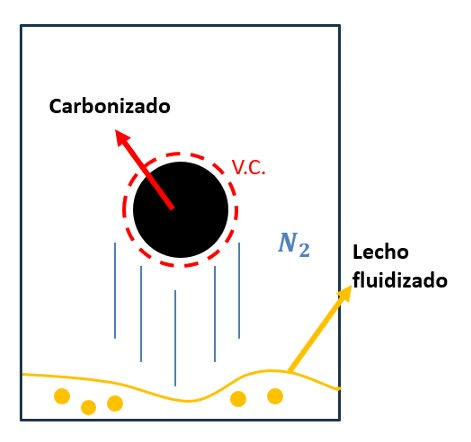
\includegraphics[width=0.35\textwidth]{figures/vc.jpg}
   \end{center}
   \caption{Volumen de control seleccionado.}
   \label{fig:vc.jpg}
\end{figure}
\medskip


\textbf{Ecuaciones gobernantes}

El comportamiento del sistema se describe mediante un conjunto de ecuaciones diferenciales obtenidas a partir de los principios de conservación.

\textbf{Conservación de la posición} 

La posición de la partícula se relaciona con su velocidad mediante:

\begin{equation}
    \frac{dz}{dt} = v
    \label{eq:dzdt}
\end{equation}

donde $z$ representa la altura de la partícula dentro del reactor y $v$ su velocidad vertical.
\medskip


\textbf{Conservación de la cantidad de movimiento} 

La ecuación de movimiento de la partícula se obtiene a partir de la segunda ley de Newton:

\begin{equation}
    m_p \frac{dv}{dt} = \sum F
    \label{eq:dvdt}
\end{equation}

Las fuerzas que actúan sobre la partícula son:

\begin{itemize}
\item Fuerza gravitacional
\item Fuerza de empuje (principio de Arquímedes)
\item Fuerza de arrastre ejercida por el gas
\end{itemize}

La fuerza gravitacional se expresa como:

\begin{equation}
    F_g = m_p g
    \label{eq:F_g}
\end{equation}

La fuerza de empuje está dada por:

\begin{equation}
    F_b = \rho_g V_p g
    \label{eq:F_bs}
\end{equation}

donde $\rho_g$ es la densidad del gas y $V_p$ el volumen de la partícula.

La fuerza de arrastre se expresa como:

\begin{equation}  
    F_D = \frac{1}{2} C_D \rho_g A_p (u_g - v)^2
    \label{eq:05}
\end{equation}

donde $C_D$ es el coeficiente de arrastre, $A_p$ el área proyectada de la partícula y $u_g$ la velocidad del gas.

Sustituyendo las fuerzas en la ecuación de movimiento se obtiene:

\begin{equation}  
    m_p \frac{dv}{dt} =
- m_p g
+ \rho_g V_p g
+ \frac{1}{2} C_D \rho_g A_p (u_g - v)^2
    \label{eq:06}
\end{equation}

Dividiendo por la masa de la partícula:

\begin{equation}  
    \frac{dv}{dt} =
- g
+ \frac{\rho_g}{\rho_p} g
+ \frac{3 C_D \rho_g}{4 \rho_p d_p}(u_g - v)^2
    \label{eq:07}
\end{equation}

\textbf{Conservación de energía} 

La variación de temperatura de la partícula se obtiene aplicando el balance de energía:

\begin{equation}  
    m_p c_p \frac{dT_p}{dt} = \dot{Q}
    \label{eq:08}
\end{equation}

El intercambio de calor ocurre por convección entre el gas y la partícula:

\begin{equation}  
    \dot{Q} = h A_p (T_g - T_p)
    \label{eq:09}
\end{equation}

Sustituyendo:

\begin{equation}  
    m_p c_p \frac{dT_p}{dt} = h A_p (T_g - T_p)
    \label{eq:10}
\end{equation}

Por lo tanto:

\begin{equation}  
    \frac{dT_p}{dt} =
\frac{h A_p}{m_p c_p}(T_g - T_p)
    \label{eq:11}
\end{equation}
\medskip

\textbf{Sistema final de ecuaciones} 

El modelo matemático queda definido por el siguiente sistema de ecuaciones diferenciales:

\begin{equation}
\begin{aligned}
\frac{dz}{dt} &= v \\
\frac{dv}{dt} &= -g + \frac{\rho_g}{\rho_p}g 
+ \frac{3C_D\rho_g}{4\rho_p d_p}(u_g - v)^2 \\
\frac{dT_p}{dt} &= \frac{hA_s}{m_p c_p}\left(T_g(z) - T_p\right)
\end{aligned}
\label{eq:sistema_final}
\end{equation}

Estas ecuaciones permiten describir simultáneamente la evolución de la posición, velocidad y temperatura de la partícula durante su recorrido en el reactor.
\medskip

\textbf{Propiedades del nitrógeno gaseoso en función de la temperatura}

Las propiedades termofísicas del nitrógeno gaseoso se modelan mediante las siguientes ecuaciones.

\paragraph{Densidad del gas $\rho_g$}
Se calcula usando la ecuación de gas ideal:

\[
\rho_g = \frac{P\,M_{N_2}}{R_u\,T}
\]

donde $M_{N_2}=0.02802\,\text{kg/mol}$ es la masa molar del nitrógeno y
$R_u=8.314\,\text{J/(mol\,K)}$ es la constante universal de los gases.

\paragraph{Viscosidad dinámica $\mu_g$}
Se calcula mediante la ley de Sutherland:

\[
\mu_g = \mu_0\left(\frac{T}{T_0}\right)^{3/2}\frac{T_0+S}{T+S}
\]

donde $\mu_0=1.663\times10^{-5}\,\text{Pa·s}$, $T_0=300\,\text{K}$ y $S=111\,\text{K}$.

\paragraph{Conductividad térmica $k_g$}
Se aproxima mediante una ley potencial:

\[
k_g = k_{\text{ref}}\left(\frac{T}{T_{\text{ref}}}\right)^{0.82}
\]

donde $k_{\text{ref}}=0.0242\,\text{W/(m\,K)}$ a $T_{\text{ref}}=273.15\,\text{K}$.

\paragraph{Capacidad calorífica $c_{p,g}$}
Se calcula a partir de un polinomio en función de la temperatura,
empleando los coeficientes reportados por NIST para el N$_2$ en el
rango de 300--1000 K.

\paragraph{Número de Prandtl $Pr$}
Se determina a partir de las propiedades anteriores:

\[
Pr = \frac{\mu_g\,c_{p,g}}{k_g}
\]
\medskip

\textbf{Coeficiente de arrastre $C_D$ --- Correlación de Schiller-Naumann}

\begin{equation}
  C_D =
  \begin{cases}
    \dfrac{24}{Re}\!\left(1 + 0.15\,Re^{0.687}\right) & \text{si } Re < 1000 \\[10pt]
    0.44 & \text{si } Re \geq 1000
  \end{cases}
  \label{eq:CD}
\end{equation}
donde $Re = \rho_g\,|v_\text{rel}|\,d_p\,/\,\mu_g$ es el número de Reynolds relativo de la partícula. Esta correlación es la base del trabajo de Almedeij (2008).
\medskip

\textbf{Coeficiente de convección $h$ --- Correlación de Ranz-Marshall}

\begin{equation}
  Nu = 2.0 + 0.6\,Re^{1/2}\,Pr^{1/3}, \qquad h = \frac{Nu\,k_g}{d_p}
  \label{eq:Nu}
\end{equation}

Válida para $0 < Re < 200$ y $0.6 < Pr < 400$. Para $Re \to 0$, $Nu \to 2$ (límite de conducción pura en esferas).

\textbf{Velocidad del gas $u_g(z)$}

A partir de la conservación de masa del gas (flujo másico constante $\dot{m} = \rho_g(T_\text{entrada})\,\dot{V}_0$):

\begin{equation}
  u_g(z) = \frac{\dot{m}}{\rho_g\!\left(T_g(z)\right)\,A(z)}, \qquad A(z) = \frac{\pi\,D(z)^2}{4}
  \label{eq:ug}
\end{equation}
\medskip

\textbf{Alcance del modelo}

El modelo desarrollado permite describir el movimiento y el calentamiento de una partícula de carbonizado transportada por un flujo de gas de nitrógeno dentro del reactor. El objetivo principal es estimar la trayectoria de la partícula y la evolución de su temperatura a lo largo del reactor, con el fin de determinar la temperatura máxima alcanzada durante el proceso.

Para simplificar el análisis, el modelo considera las siguientes características:

\begin{itemize}
\item El sistema se analiza mediante el seguimiento de una partícula representativa.
\item El movimiento de la partícula se considera unidimensional en dirección vertical.
\item El intercambio de calor entre el gas y la partícula ocurre únicamente por convección.
\item Las propiedades de la partícula se consideran constantes.
\item Las propiedades del gas dependen de la temperatura local del reactor.
\item El perfil de temperatura del gas se obtiene a partir de los datos experimentales registrados por las termocuplas.
\end{itemize}
\medskip

\subsection{Suposiciones y simplificaciones del modelo}

Con el fin de desarrollar un modelo matemático que describa el comportamiento dinámico de una partícula de carbonizado durante su recorrido en el reactor de lecho fluidizado, se establecieron una serie de suposiciones y simplificaciones. Estas permiten reducir la complejidad del sistema real y facilitan la formulación y solución de las ecuaciones gobernantes.

\begin{itemize}

\item \textbf{La partícula de carbonizado se modela como una esfera rígida:}  
Se asume que la partícula posee geometría esférica con diámetro constante de $150\,\mu m$, lo cual simplifica el cálculo del área superficial, volumen y coeficientes de transferencia.

\item \textbf{Las propiedades físicas de la partícula son constantes:}  
La densidad de la partícula ($\rho_{carb} = 810\,kg/m^3$) se considera constante durante todo el proceso, despreciando posibles cambios estructurales o de masa durante la pirólisis.

\item \textbf{El gas de fluidización es nitrógeno ideal:}  
El nitrógeno se modela como un gas ideal, por lo que sus propiedades termodinámicas pueden estimarse mediante relaciones estándar dependientes de la temperatura.

\item \textbf{El flujo de gas en el reactor se considera unidimensional:}  
Se supone que la velocidad del gas varía únicamente en la dirección axial del reactor y se desprecia cualquier variación radial o turbulencias locales.

\item \textbf{La partícula experimenta únicamente fuerzas de arrastre y gravedad:}  
En el balance de fuerzas se consideran solamente la fuerza gravitacional y la fuerza de arrastre ejercida por el gas, despreciando efectos como colisiones con otras partículas o fuerzas de flotación complejas.

\item \textbf{La temperatura del gas se aproxima mediante interpolación entre las termocuplas:}  
Las temperaturas medidas en los puntos PT1, PT2, PT3 y PT4 se utilizan para aproximar el perfil de temperatura del gas a lo largo del reactor.

\item \textbf{Transferencia de calor dominante por convección:}  
Se asume que el principal mecanismo de transferencia de calor entre el gas caliente y la partícula es la convección, mientras que la radiación térmica se desprecia debido al pequeño tamaño de la partícula.

\item \textbf{Temperatura uniforme dentro de la partícula:}  
Se considera que la partícula posee temperatura uniforme en todo su volumen (modelo de capacidad concentrada), lo cual es válido cuando la resistencia interna a la conducción es pequeña comparada con la resistencia convectiva externa.

\item \textbf{No ocurre transferencia de masa:}  
El modelo se enfoca únicamente en el análisis de transferencia de calor y dinámica de la partícula, por lo que no se consideran reacciones químicas adicionales ni pérdida de masa durante el recorrido.

\item \textbf{Condiciones de presión constantes:}  
La presión del sistema se mantiene constante en aproximadamente $1\,atm$ durante todo el proceso de fluidización.
\end{itemize}
\medskip

\subsection{Implementaci\'on Computacional}
El sistema de tres EDOs acopladas (\cref{eq:sistema_final})
se resolvió numéricamente mediante el método de \textbf{Runge-Kutta de cuarto
orden (RK4)}, implementado desde cero en Python. Este método pertenece a la
familia de métodos de un paso y se construye a partir de cuatro evaluaciones
de la función $\mathbf{f}(t, \mathbf{y})$ por cada avance de tiempo, lo que
le confiere un error de truncamiento local de orden $\mathcal{O}(h^5)$ y un
error global de orden $\mathcal{O}(h^4)$, siendo $h$ el tamaño del paso.

Dado el sistema en forma vectorial:
\begin{equation}
    \frac{d\mathbf{y}}{dt} = \mathbf{f}(t,\, \mathbf{y}), \qquad
    \mathbf{y} = \begin{pmatrix} z \\ v \\ T_p \end{pmatrix}, \qquad
    \mathbf{f} = \begin{pmatrix} v \\ dv/dt \\ dT_p/dt \end{pmatrix}
    \label{eq:sistema_vectorial}
\end{equation}

el avance desde el instante $t_n$ hasta $t_{n+1} = t_n + h$ se calcula
evaluando $\mathbf{f}$ en cuatro puntos distintos del intervalo, combinados
con pesos específicos:

\begin{align}
    \mathbf{k}_1 &= \mathbf{f}\!\left(t_n,\; \mathbf{y}_n\right)
    \label{eq:k1}\\
    \mathbf{k}_2 &= \mathbf{f}\!\left(t_n + \tfrac{h}{2},\;
                    \mathbf{y}_n + \tfrac{h}{2}\,\mathbf{k}_1\right)
    \label{eq:k2}\\
    \mathbf{k}_3 &= \mathbf{f}\!\left(t_n + \tfrac{h}{2},\;
                    \mathbf{y}_n + \tfrac{h}{2}\,\mathbf{k}_2\right)
    \label{eq:k3}\\
    \mathbf{k}_4 &= \mathbf{f}\!\left(t_n + h,\;
                    \mathbf{y}_n + h\,\mathbf{k}_3\right)
    \label{eq:k4}
\end{align}

\begin{equation}
    \mathbf{y}_{n+1} = \mathbf{y}_n
    + \frac{h}{6}\left(\mathbf{k}_1 + 2\,\mathbf{k}_2
                      + 2\,\mathbf{k}_3 + \mathbf{k}_4\right)
    \label{eq:rk4_avance}
\end{equation}

Cada pendiente $\mathbf{k}_i$ tiene una interpretación física concreta:
$\mathbf{k}_1$ es la pendiente al inicio del intervalo;
$\mathbf{k}_2$ y $\mathbf{k}_3$ son estimaciones en el punto medio usando
las pendientes anteriores como predictor; y $\mathbf{k}_4$ es la pendiente
al final del intervalo. El promedio ponderado de la \cref{eq:rk4_avance}
asigna mayor peso a las estimaciones del punto medio ($2\mathbf{k}_2$ y
$2\mathbf{k}_3$), lo que da origen al orden de convergencia cuarto.

El algoritmo implementado opera con un \textbf{paso fijo} $h = 10^{-5}$ s,
valor seleccionado para capturar con precisión el transitorio inicial de
aceleración de la partícula (primeros 5--10 ms), donde las derivadas de
velocidad son más pronunciadas. La integración avanza paso a paso hasta
cumplir una de dos condiciones de parada: que el tiempo supere $t_f$, o
que la partícula alcance la altura máxima del reactor $z_{max} = 1.12$ m.
La \cref{fig:diagrama} presenta el diagrama de flujo completo.


\subsection{Resultados}
Se sugiere tener una secci\'on dedicada exclusivamente a la presentaci\'on de
los resultados obtenidos, as\'i como a la discusi\'on de tendencias
observadas(a partir de los resultados), o a la observaci\'on de comportamientos
que puedan ser considerados an\'omalos o contrarios a las observaciones
documentadas por la bibliograf\'ia.  Igualmente, es indispensable que todas las
gráficas y curvas incluidas en el informe tengan una resolución adecuada, y las
etiquetas e indicadores de escalas, as\'i como t\'itulos de gr\'aficos, tengan
un tama\~no adecuado para una f\'acil lectura, como se muestra en el ejemplo de
la \cref{fig:dflujo}

\begin{figure}[!hbt]
    \begin{center}
        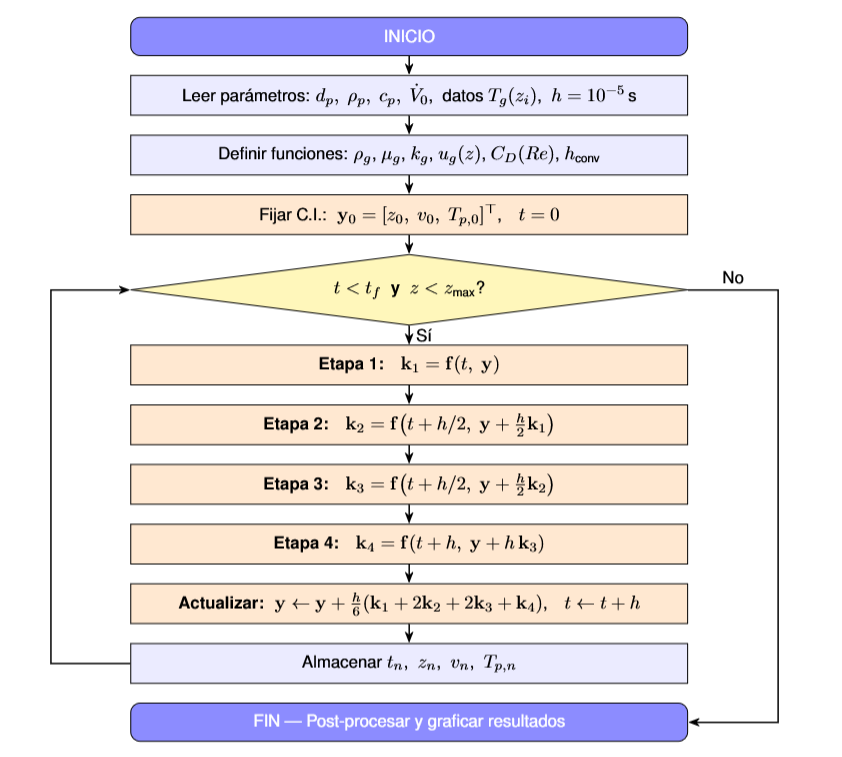
\includegraphics[width=0.75\textwidth]{figures/dflujo.PNG}
    \end{center}
    \caption{Diagrama de flujo del allgoritmo solución}
    \label{fig:dflujo}
\end{figure}

\subsection{Conclusiones}
Cada uno de los casos deber\'a tener una secci\'on de conclusiones donde se
discutan las principales observaciones y hallazgos obtenidos mediante el uso de
modelo matem\'atico-computacional, o del modelo matem\'atico-anal\'itico (si
ese fuese el caso).  Las conclusiones podr\'an incluir apreciaciones acerca de
dificultades en la construcci\'on del modelo, o en la implementaci\'on
computacional que se haya hecho. En cualquier caso, se dar\'a m\'as importancia
a la presentaci\'on de discusiones asociadas al comportamiento del sistema,
fen\'omeno, o proceso explorado en el caso en cuesti\'on. Se evaluar\'a de
manera MUY negativa cualquier tipo de discusi\'on que carezca de
fundamentaci\'on o de apoyo en los resultados presentados en el informe.

\lipsum[1-2]

\section{BIBLIOGRAFÍA}


\end{document}          
